\documentclass[12pt]{article}
\usepackage{lingmacros}
\usepackage{tree-dvips}
\usepackage{multicol}
\usepackage{graphicx}
\usepackage[section]{placeins}
\usepackage{hyperref}
\usepackage{caption}
\usepackage{listings}
\usepackage{indentfirst}


\hypersetup{
	colorlinks=true,
	linkcolor=blue,
	filecolor=magenta,      
	urlcolor=cyan,
}
\title{\Huge \bfseries \emph{Assignment 3}}
\author{Vathana Him}
\date{November 25, 2021}


\begin{document}
\maketitle
\section{Abstract}
\hspace*{5mm} The purpose of this assignment is to use the data of the image created from assignment 1 to build classification models in a distributed system in databricks in order to classify the choosen images
and compare the results and run time to that of the model built in our local machine. This assignment utilized images from UCI respository as sample datasets that will be used to train a machine learning model. 
Images that were processed represented three fruits spanish pear, fuji apple, watermelon. These images were labeled as Image0, Image1, and Image2 respectively and their dataset was processed and dervied in assignment1 for both the non-overlapping and 
overlapping layer. These labels was then encoded to take in the values of 0, 1, and 2. The primary machine learning that was used in order to classify these images was random forest. Prior to training the machine learning model,
additional methods were taken into account in feature selection and data scaling in order to reduce the size of the data and train the model with a sufficient outcome.
The random forest model in databricks was then used to compare to the random forest model that was dervied in our local machine in assignment2. 

\begin{multicols*}{2}
  \section{Task 1}
  \hspace*{5mm} In assignment1, the three images were divided into 8X8 pixel blocks, the grayscale images were then divided into sliding block of 8X8 pixels. Each feature was then assigned a label respectively to identify them. 
  Two helper functions were used for this task, sliding blocks feature function which converts an image into sliding image blocks given an image object, and 
  label feature function which create feature labels for each image given a list that contains the array of sliding images. The dimension of the gray images were resized to height of 256 and width of 344. The purpose for these choosen dimensions was to keep its aspect ratio. 
  Additionally, the resized height and width must also be divible by eight since this project divided the targeted image into sliding blocks and non-sliding blocks of 8 by 8 height and width. T
  he feature vector that was constructed from these images created 6800 feature vectors for the sliding block and 3400 feature vectors for the non-sliding block and each feature vector lies a 8 by 8 pixels who’s value lies between 0-255 of the gray image scale. 
  The features of each feature vector was then flatten to 64 features for each respective feature vector. These datasets was exported into cvs files in the data folder.
  The evidence of this dataset can be shown in 2.1 Figure 1. 

  \subsection{Assignment 1 Figure} 
	\begin{center}
		\captionof{figure}{CVS Data Folder}
		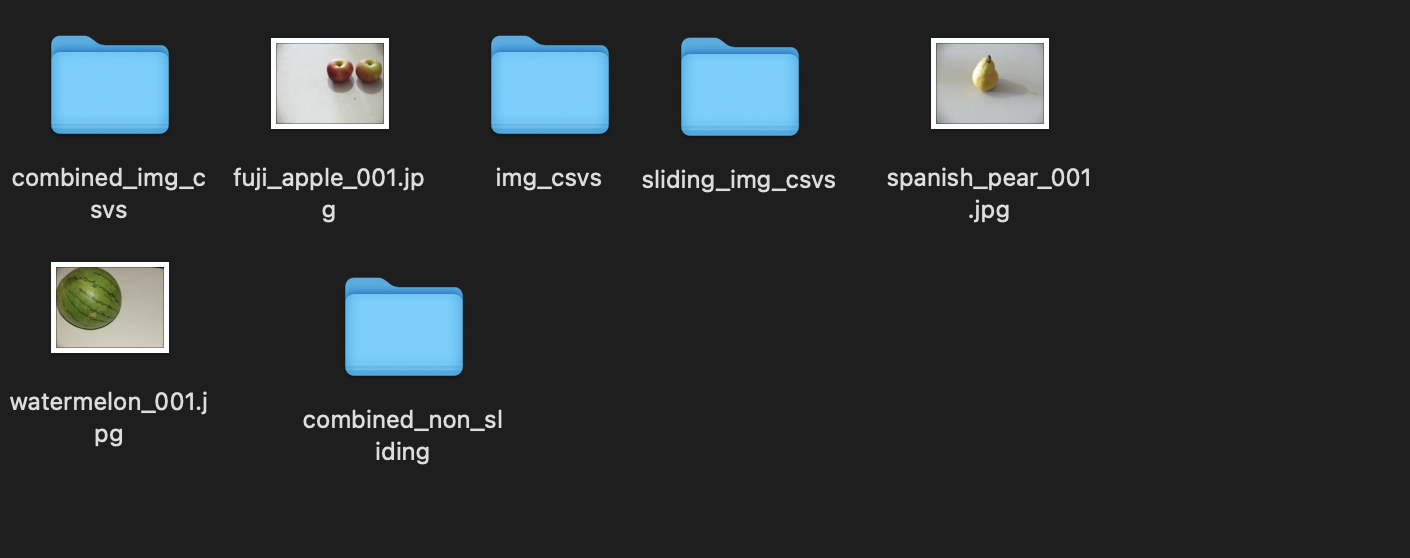
\includegraphics[scale=0.2]{../screenshot/csvs.png}	
    \end{center}


  \hspace*{5mm} In assignment2, the random forest classifier was used to classify the images of different set in non-overlapping image01, 
  overlapping image01, non-overlapping image012, and overlapping image012. Feature selection was also used in this model to increase
  the speed of the training time and reduce the computational power. The select from model feature selection from Sklearn compare the average
  importance of all features at a threshold value and dropped features that were below the threshold. Additionally the elastic net model will also be presented. However, the random forest models
  will only be used to compare with the databricks model. 

  \hspace*{5mm} In the two class classification for non-overlapping image0 and image1, the training accuracy score was 0.95 and the testing 
  accuracy score was 0.92 based on 2.2 Figure 2. There was not a significant difference between the train and test score, this suggests that the train-test split 
  provided a well balanced data between the two classes. The confusion matrix in 2.2 Figure 3 confirmed a true prediction value of 240 and false prediction value of 
  32 for class 0 and a true prediction value of 269 and false prediction value of 10 for class 1. This indicate that the accuracy rate and the precision
  rate for class 0 and class 1 was relatively as seen in 2.2 Figure 4 of the derived accuracy score and precision for both class 0 and class 1 respectively.
  Class 0 had a precision rate of 0.92, while class 1 had a precision rate of 0.89. This model provided a good accruacy for each of the predicted classes.

  \subsection{Assignment 2 Figure} 
  \begin{center}
      \captionof{figure}{Non-Overlapping Image01 RF Score}
		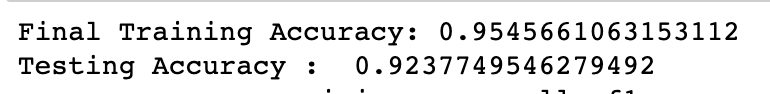
\includegraphics[scale=0.5]{../screenshot/Rf-Non-Overlapping01/score.png}

        \captionof{figure}{Non-Overlapping RF Confusion-Matrix}
            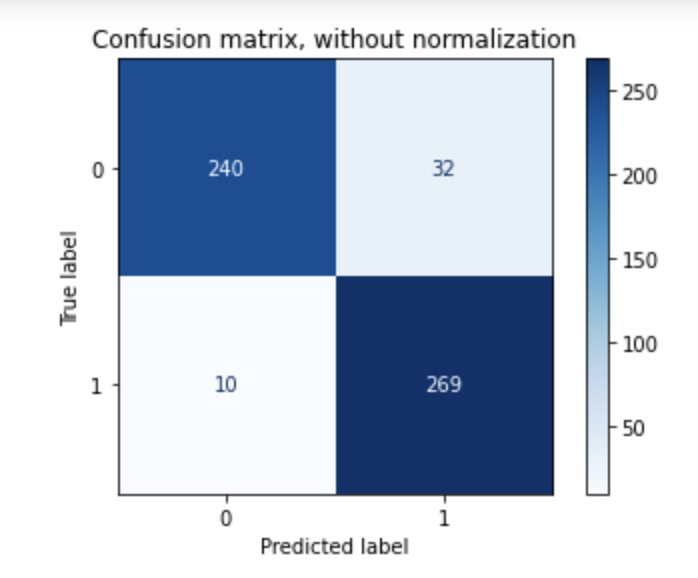
\includegraphics[scale=0.5]{../screenshot/Rf-Non-Overlapping01/cf.png}

        \captionof{figure}{Non-Overlapping RF Derived Score}
        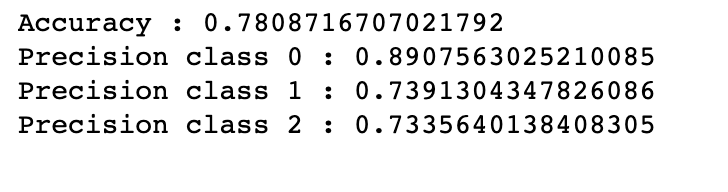
\includegraphics[scale=0.5]{../screenshot/Rf-Non-Overlapping012/calc_score.png}
  \end{center}

  \hspace*{5mm} For the overlapping two-class classificaion of image0 and image1, the training accruacy score was ~0.96 and the testing
  accuracy score was 0.92 based on 2.3 Figure 5. This small difference in accuracy score indicates that the train-test split provided an evenly balanced data for the test and train
  set for the random forest model. The confusion matrix on 2.3 Figure 6 provided the result of the test set as class 0 had 590 true prediction and 74 false prediction,
  while class 1 had 666 true prediction and 30 false prediction. This indicated a high precision value for both class 0 and class 1 because the model
  was able to make a prediction of the two images at a high accuracy rate. Based on the value of this confusion matrix, the hand calculation for accuracy score,
  precision for class 1 and precision for class 0 was derived. In 2.3 Figure 7, the accuracy score from the dervied calculation was 0.92 with a precision of 0.95 and 0.9
  for class 0 and class 1 respectively. Based on these high precision values, it indicated that this model can be produced the same results when test with another
  dataset of the same characteristics. This model also performed significantly better than the elstaic-net for two-class classification of overlapping
  image0 and image1. 

  \subsection{Assignment 2 Figure} 
  \begin{center}
        \captionof{figure}{Over-lapping Image01 RF Score}
        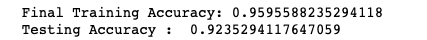
\includegraphics[scale=0.5]{../screenshot/Rf-Overlapping01/score.png}

        \captionof{figure}{Over-lapping RF Confusion-Matrix}
        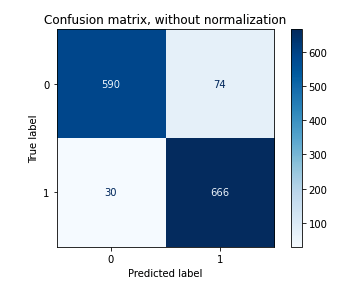
\includegraphics[scale=0.5]{../screenshot/Rf-Overlapping01/cf.png}

        \captionof{figure}{Over-lapping RF Derived Score}
        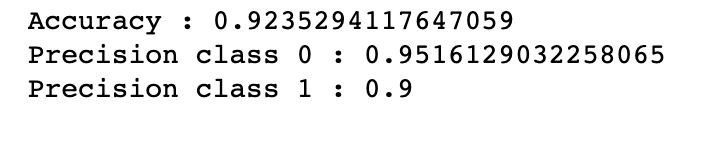
\includegraphics[scale=0.5]{../screenshot/Rf-Overlapping01/calc_score.png}

  \end{center}

  \hspace*{5mm} In the non-overlapping elastic model, the data for non-overlapping image01 was used. The result of the model for
  non-overlapping image01 yielded a training accuracy of 0.69 and testing accuracy of 0.67 as shown in 2.4 Figure 8. A similar 
  score in both the train and test set indicate that the data was balanced between the train and test set. The confusion matrix in 2.4 
  Figure 9 indicate that there were 197 predictions of True Positive for class 0 and 175 predictions of True Positive for class 1. These
  results was then used to manually derived the accuracy and precision. According to the manual derivated result in 2.4 Figure 10, the overall
  accuracy of the model was 0.72 with a precision of 0.72 for class 0 and 0.72 for class 1. This accuracy score indicate that there was a sufficient
  number of true postives for class 0 and class 1. However, the number of false postives was still indicative in affecting the accuracy score.


  \subsection{Assignment 2 Figure} 
  \begin{center}

    \captionof{figure}{Non-Overlapping Image01 Elastic-Net}
    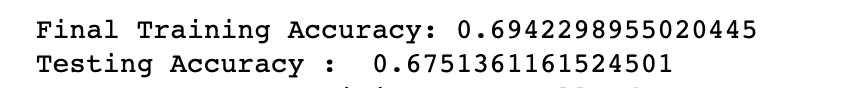
\includegraphics[scale=0.5]{../screenshot/Non-Overlapping-Elastic-results/results.png}

    \captionof{figure}{Non-Overlapping Image01 Elastic-Net Confusion-Matrix}
    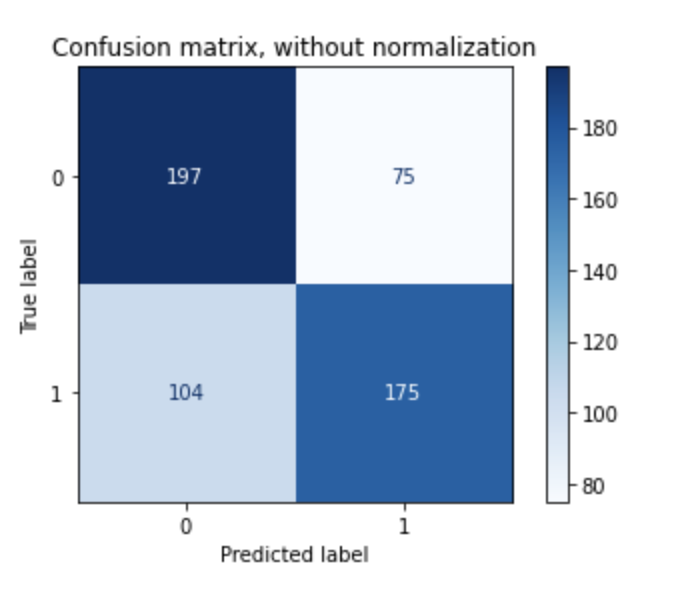
\includegraphics[scale=0.5]{../screenshot/Non-Overlapping-Elastic-results/cf.png}

    \captionof{figure}{Non-Overlapping Image01 Elastic-Net Derived Score}
    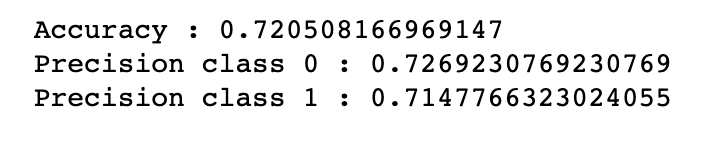
\includegraphics[scale=0.5]{../screenshot/Non-Overlapping-Elastic-results/calc_score.png}

  \end{center}

  \hspace*{5mm} In the second elastic model, the data for overlapping image01 was used. The result of the model for overlapping
  image01 resulted in a training accuracy of 0.60 and a testing accuracy of 0.59. This inidcated that the data had a great degree of
  randomeses and it was balanced in the train-test set. The confusion matrix in 2.5 Figure 11 resulted in 493 prediction of true prediction 
  and 314 of true prediction for class 0 and 1 respectively. However, in the derived precision score for class 0 was relatively lower than that
  of class 1 as shown in 2.5 Figure 12. This could indicate that there was an imbalance in the dataset between class 0 and class 1. Additionally, because of the nature of the
  image choosen, the black and white image of apple and pear had similar texture and texture. The overlapping nature of the dataset could distort the elastic-net loss function, 
  when it attempted to classify the two images. This also impacted the overall dervied accuracy score of the model with a value of 0.65 as shown in 
  2.5 Figure 13. An accuracy score of 0.65 indicate that this model was not sufficient enough for making a prediction. 


  \subsection{Assignment 2 Figure} 
  \begin{center}

    \captionof{figure}{Overlapping Image01 Elastic-Net}
    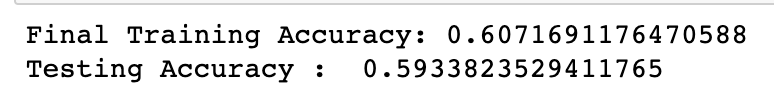
\includegraphics[scale=0.5]{../screenshot/Overlapping-Elastic-results/results.png}

    \captionof{figure}{Overlapping Image01 Elastic-Net Confusion-Matrix}
    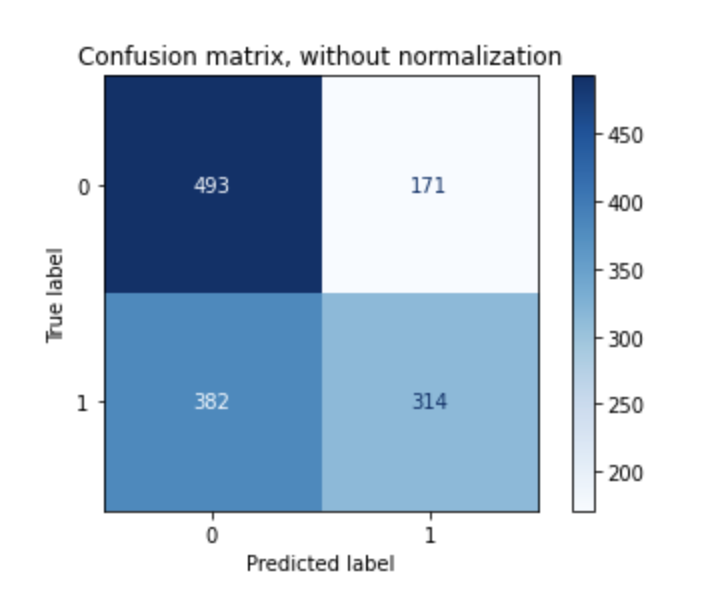
\includegraphics[scale=0.5]{../screenshot/Overlapping-Elastic-results/cf.png}

    \captionof{figure}{Overlapping Image01 Elastic-Net Derived Score}
    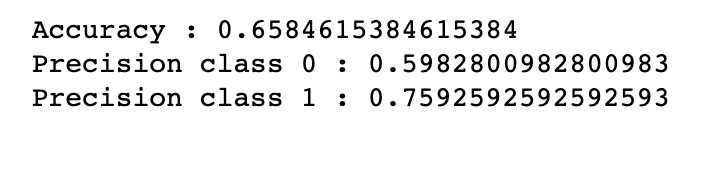
\includegraphics[scale=0.5]{../screenshot/Overlapping-Elastic-results/hand_score.png}

  \end{center}

  \hspace*{5mm} In contrast to the two-class non-overlapping classification random forest, the three-class
  classification of image0, image1 and image2 testing and training accuracy score deviate in larger degree.
  In 2.6 Figure 14, the training accuracy for this model is 0.89, whereas the testing accuracy for this model is 
  0.78. This may indicate an overfit in the model and that the train-test split set did not generate a well balanced enough data.
  The confusion matrix in 2.6 Figure 15 showed that a true prediction value of 212 for class 0, 221 for class 1, and 212 for class 2.
  These values was then used to dervied the caculated precision for each of the class. 2.6 Figure 16 indicated that class 0 had a 0.89 precision,
  class 1 had a precision of 0.74 and class 2 ha da precision of 0.73. The difference in this precision score can suggest that the model
  was overfitted to favor class 0. 


  \subsection{Assisgnment 2 Figures} 
	\begin{center}
    \captionof{figure}{Non-Overlapping Image012 RF Score}
		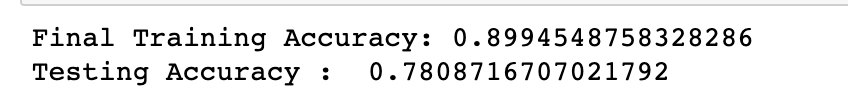
\includegraphics[scale=0.5]{../screenshot/Rf-Non-Overlapping012/score.png}

    \captionof{figure}{Non-Overlapping Image012 RF Confusion-Matrix}
		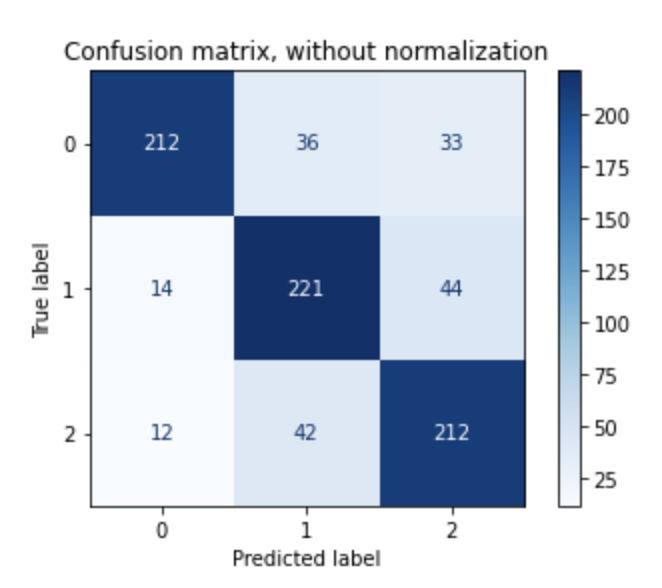
\includegraphics[scale=0.5]{../screenshot/Rf-Non-Overlapping012/cf.png}

    \captionof{figure}{Non-Overlapping Image012 RF Derived Score}
		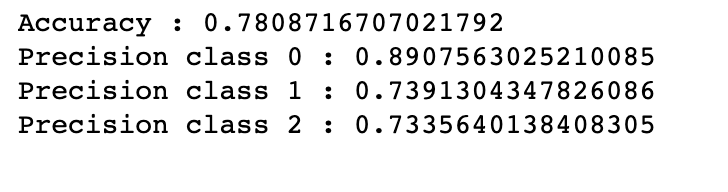
\includegraphics[scale=0.5]{../screenshot/Rf-Non-Overlapping012/calc_score.png}
	\end{center}


  \hspace*{5mm} Similar to the three-class non-overlapping random forest model, the three-class classification of overlapping 
  image0, image1 and image2 testing and training accuracy score also deviated to a noticeable extent.
  In 2.7 Figure 17, the training accuracy for this model is 0.91, whereas the testing accuracy for this model is 
  0.83. This may indicate a slight overfit in the model and that the train-test split set did not generate a well balanced enough data.
  The confusion matrix in 2.7 Figure 18 showed that a true prediction value of 552 for class 0, 608 for class 1, and 545 for class 2.
  These values was then used to dervied the caculated precision for each of the class. 2.7 Figure 19 indicated that class 0 had a 0.94 precision,
  class 1 had a precision of 0.77 and class 2 ha da precision of 0.81. The difference in this precision score can suggest that the model
  was overfitted to favor class 0, which is similar to that of the three-class random forest non-overlapping model. Although the dataset was 
  randomly shuffled, the training set may have contained slightly more data for class 0 than that of class 2 and class 1.  

  \subsection{Assisgnment 2 Figures} 
  \begin{center}
    \captionof{figure}{Overlaping Image012 RF Score}
		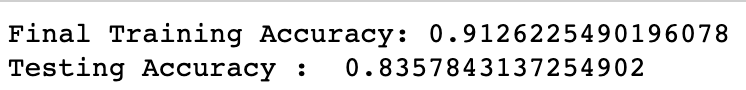
\includegraphics[scale=0.5]{../screenshot/Rf-Overlapping012/score.png}

    \captionof{figure}{Overlapping Image012 RF Confusion-Matrix}
		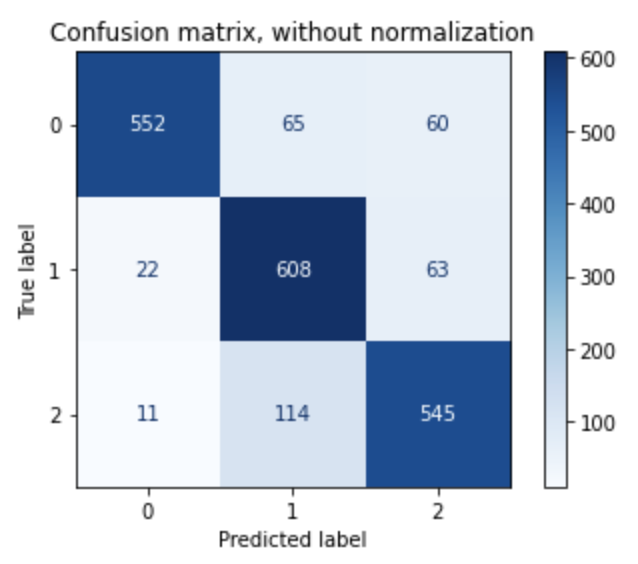
\includegraphics[scale=0.5]{../screenshot/Rf-Overlapping012/cf.png}

    \captionof{figure}{Overlapping Image012 RF Derived Score}
		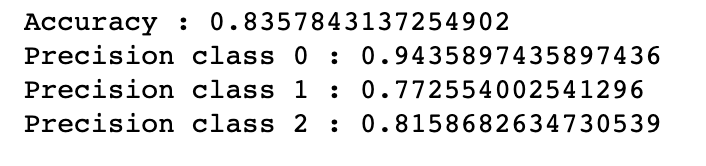
\includegraphics[scale=0.5]{../screenshot/Rf-Overlapping012/calc_result.png}
  \end{center}

  \section{Task 2 (Knowledge Gained)}
  \hspace*{5mm} The purpose of this task is to explained the knowledge gained through databricks "Explore the Quickstart Tutorial Section".\footnote[1]{https://docs.databricks.com/getting-started/quick-start.html}.
  Databricks seems to be a cloud-based platform that can run ETL processes for processing and transforming large quantities of data for machine learning models. 
  Databrick has a network of distributed systems that allows it to handle big quantities of data without any time loss through its system. 
  These distributed systems are powered by third-party cloud providers such as Google Cloud, Azure Web Services, and Amazon Web Services. 
  For example in the quick start tutorial, the dataset that was used was stored in a Databricks dataset directory, which used the storage engine of Amazon Web Services. 
  Instead of storing it locally, this dataset is stored on the cloud that is provided by Amazon Web services as this method of storage can handle millions of terabytes of data in theory. 
  In the quick start tutorial, the notebook exported the data from a dataset that was stored in an Amazon Web Services storage and loaded through a cloud computing cluster 
  that is also provided by Amazon Web Services. When these services are integrated, the notebook works as if you’re working on your local machine notebook.


  \hspace*{5mm} You can load the dataset, process the dataset to draw insights and analysis as well as train machine learning models. 
  Additionally, the notebook can be chosen to work with specific instances of a data language. These instances can include pyspark, python, sql and scala. 
  The integration of multiple data processing languages in a singular cluster of computing resource that is provided by the users chosen cloud service provider can offer a seemly effortless workflow that allows users to work, 
  integrate, and build machine learning model flows as well as performing extract, load, and transformation processes to a data storage platform that is not dependent on a local computing power. 
  This will not confine a user's big data project to a single local computer resource and will speed up the processing power of end-to-end machine learning model flows through the use of cloud computing clusters.  

  \hspace*{5mm} This method of processing and storing data can be coined the term “data lake” and “data warehouse” as databases provide a service of cloud data platform that 
  leverages the cloud service of cloud providers such as Google Cloud, Azure Web Services, and Amazon Web Services. This type of architecture was based on an open source 
  Apache Spark framework that allows users to query against semi-structured data without having to use the traditional database schema for the purpose of speed and efficiency. 
  Since cloud storage and cloud computing (clusters) are used, the limited source of on-prem computing resources is no-longer a detriment to working with massive amounts of data. 

  \hspace*{5mm} In order to set up databricks for Task 3, the following steps was done. Databricks was connected to an Amazon Web Services account in order to use their storage system as well as their EC2
  cloud computing to generate the needed custer of cpu resources. When Amazon Web Services was connected, the cpu cluster was configured. The configured clusters had the following specs 7.3 LTS 
  (includes Apache Spark 3.0.1, Scala 2.12) as seen in 3.1 Figure 20. The data is then loaded into the DBFS, which is backed by AWS storage as shown in 3.1 Figure 21. 

  \subsection{Task 2 Figures}
  \begin{center}
  \captionof{figure}{Configured CPU Cluster}
	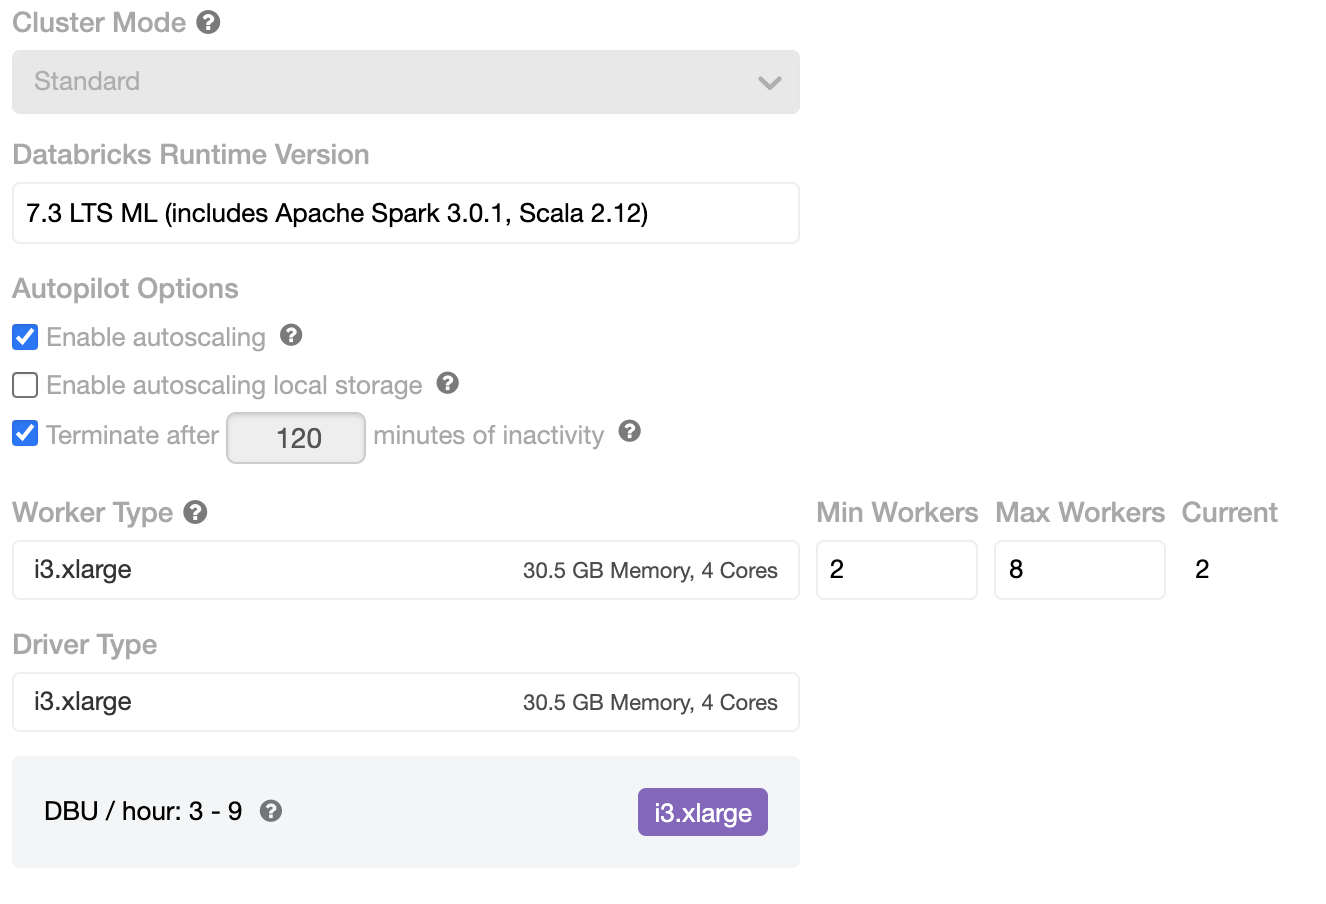
\includegraphics[scale=0.4]{../screenshot/cpu_cluster.png}

  \captionof{figure}{Loaded Data}
	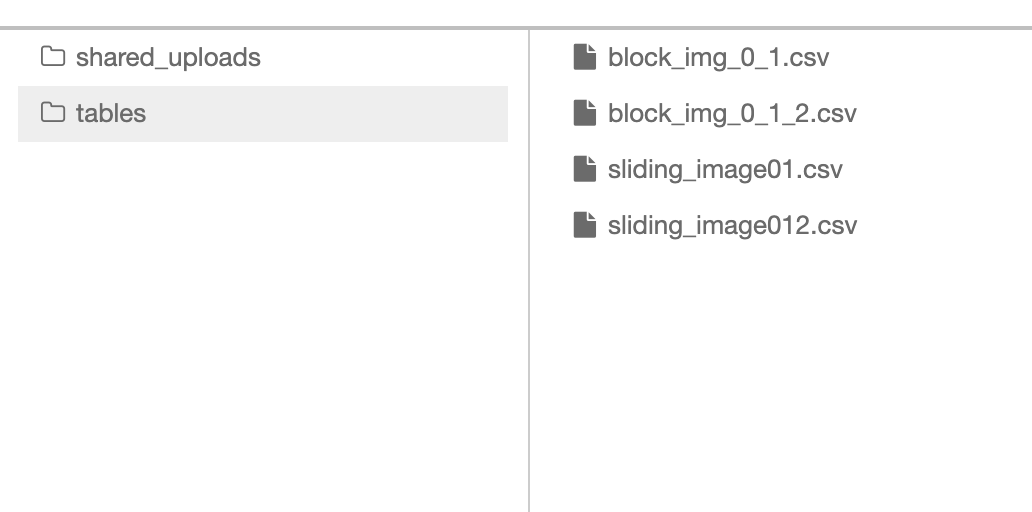
\includegraphics[scale=0.4]{../screenshot/dataload.png}
  \end{center}


  \section{Task 3}
  \hspace*{5mm} In Task 3, the random forest multi-class classifier was implemented in Databricks datastributed system with backend support from 
  the cpu cluster and storage capcacity of Amazon Web Services EC2 and S3. The code that was implemented had charactertistics of the code from assignment2 through the use
  of random forest classification to classify three choosen images in fuji apple, pear, and watermelon. These images were labeled image0, image1 and image2 respectively. In the data pre-processing
  step of this task, an analysis of the dataset for non-overlapping image01, overlapping image01, non-overlapping image012, and overlapping image012 was done. It was seen that the number of class label
  for each image was equally distributed for both the overlapping and non-overlapping set as shown in 4.1 Figure 24 and Figure 25. This indicate that there was no imbalance of classes among the dataset.
  Subsequently, the distribution of the dataset was analzyed among all the feature space of feature 54 to determine if anything scaling is needed. It can be seen that in the 4.1 boxplots of Figure 23, Figure 25, 
  Figure 27, and Figure 29, the data among the three classes of overlapping and non-overlapping images as well as the two classes of overlapping and non-overlapping images contain outliers and non-normally distributed data. 
  From this finding, a scaling of min-max for each respective dataset was used before it was fed into the random forest machine learning model. Finally, since we are training on a large distributed system all features of the 
  dataset was used since we're not limited by the computation powers of our local machine. 

  \subsection{Task 3 Figures Preprocessing}
  \begin{center}
  \captionof{figure}{Non-Overlaping Image01 distribution}
	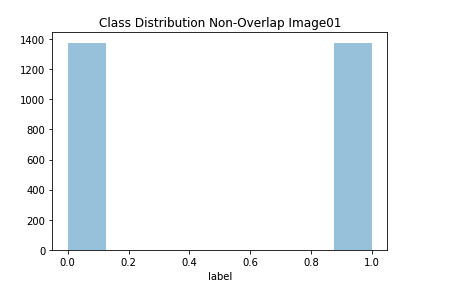
\includegraphics[scale=0.4]{../screenshot/Pre-Non-Overlapping/dist01.png}

  \captionof{figure}{Non-Overlaping Image01 boxplot}
	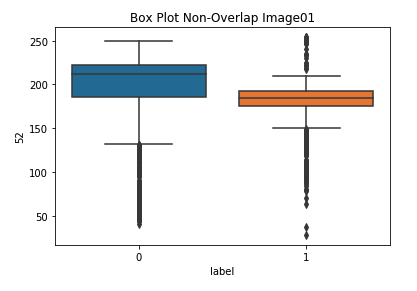
\includegraphics[scale=0.4]{../screenshot/Pre-Non-Overlapping/box01.png}

  \captionof{figure}{Non-Overlaping Image012 distribution}
	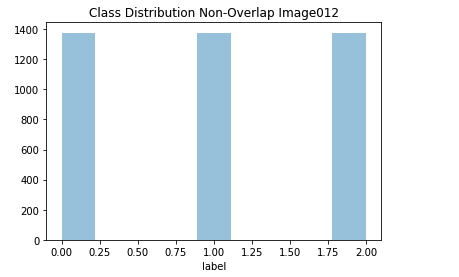
\includegraphics[scale=0.4]{../screenshot/Pre-Non-Overlapping/dis012.png}

  \captionof{figure}{Non-Overlaping Image012 boxplot}
	\includegraphics[scale=0.4]{../screenshot/Pre-Non-Overlapping/box012.png}

  \captionof{figure}{Overlaping Image01 distribution}
	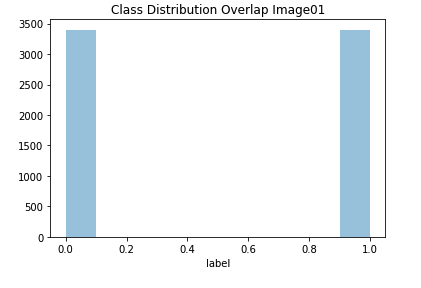
\includegraphics[scale=0.4]{../screenshot/Pre-Overlapping/dist01.png}

  \captionof{figure}{Overlaping Image01 boxplot}
	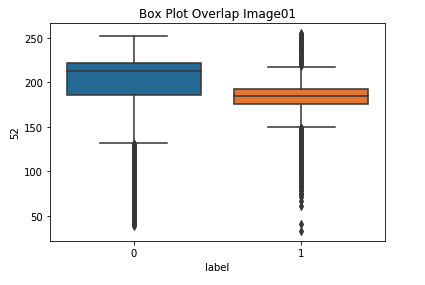
\includegraphics[scale=0.4]{../screenshot/Pre-Overlapping/box01.png}

  \captionof{figure}{Overlaping Image012 distribution}
	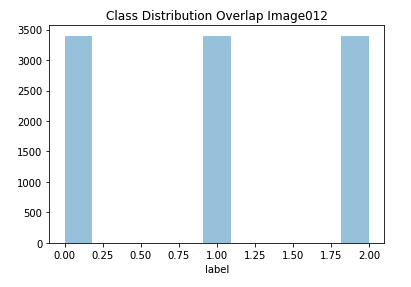
\includegraphics[scale=0.4]{../screenshot/Pre-Overlapping/dist012.png}

  \captionof{figure}{Overlaping Image012 boxplot}
	\includegraphics[scale=0.4]{../screenshot/Pre-Overlapping/box012.png}
  \end{center}

  \hspace*{5mm} The random forest machine learning model implemented in databricks for non-overlapping image01 provided very good results in terms of numeric
  accuracy and precision measurements. In 4.2 Figure 30, the final training accuracy was 0.95 and testing accuracy was ~0.92. This suggested that the splitting of training and testing data provided an equally
  balanced data for the model to use. Additionally, class0 and class1 had a precision rate of 0.96 and 0.89 respectively, which produces very high true-poistives values for the respective classes. 
  The ROC curve in 4.2 Figure 32 also provided a very high rate of true positive to low false postitive based on the auc value of 0.92. This indicate a very high rate of accurate prediction among 
  the two classes.



  \subsection{Task 3 Figures Non-Overlapping Image01}
  \begin{center}
  \captionof{figure}{Non-Overlaping Image01 Score}
	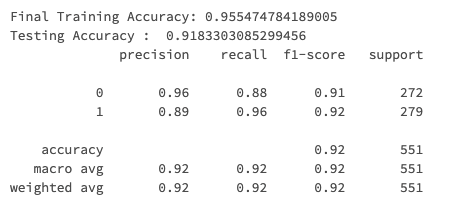
\includegraphics[scale=0.4]{../screenshot/Non-Overlapping/score01.png}

  \captionof{figure}{Non-Overlaping Image01 Confusion Matrix}
	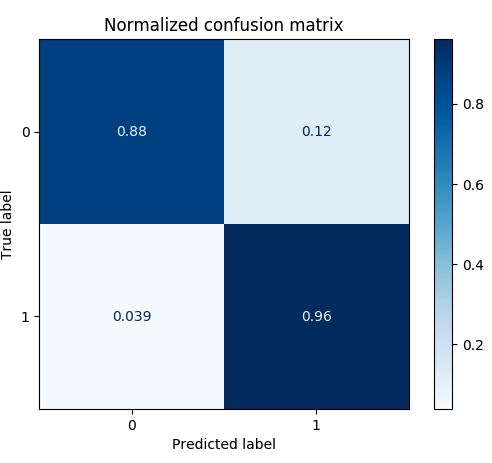
\includegraphics[scale=0.3]{../screenshot/Non-Overlapping/cf01.png}

  \captionof{figure}{Non-Overlaping Image01 ROC Curve}
	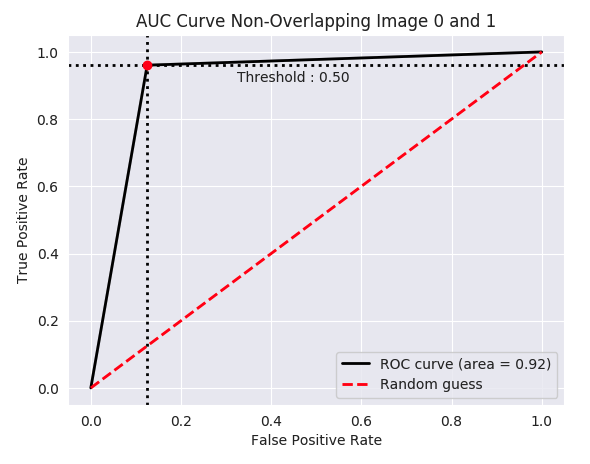
\includegraphics[scale=0.3]{../screenshot/Non-Overlapping/roc01.png}
  \end{center}


  \hspace*{5mm} In comparision, the random forest machine learning model implemented in databricks for overlapping image01 and overlapping image01 also provided very good results in terms of numeric
  accuracy and precision measurements. In 4.3 Figure 33, the final training accuracy was 0.97 and testing accuracy was 0.92. This suggested that the splitting of training and testing data provided an equally
  balanced data for the model to use. Additionally, class0 and class1 had a precision rate of 0.95 and 0.90 respectively, which produces very high true-poistives values for the respective classes. 
  The ROC curve in 4.3 Figure 35 also provided a very high rate of true positive to low false postitive based on the auc value of 0.92. This indicate a very high rate of accurate prediction among 
  the two classes. The result of the random forest model for the two class dataset for overlapping and non-overlapping images provided nearly identical results, which indicate that this model can be a 
  good predictor of a two class fruit dataset.

  \subsection{Task 3 Figures Overlapping Image01}
  \begin{center}
  \captionof{figure}{Overlaping Image01 Score}
	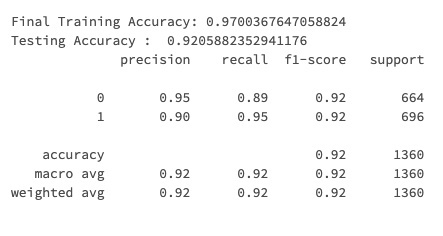
\includegraphics[scale=0.4]{../screenshot/Overlapping/score01.png}

  \captionof{figure}{Overlaping Image01 Confusion Matrix}
	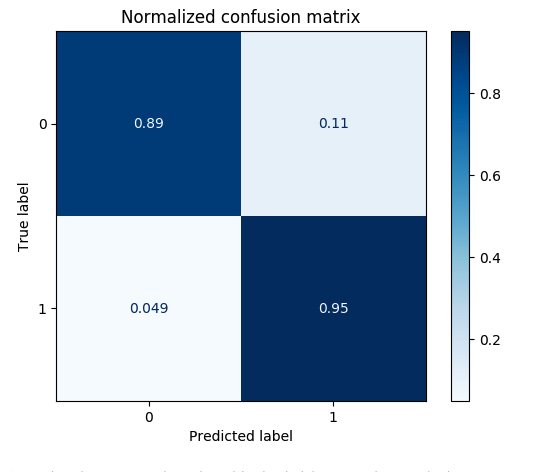
\includegraphics[scale=0.3]{../screenshot/Overlapping/cf01.png}

  \captionof{figure}{Overlaping Image01 ROC Curve}
	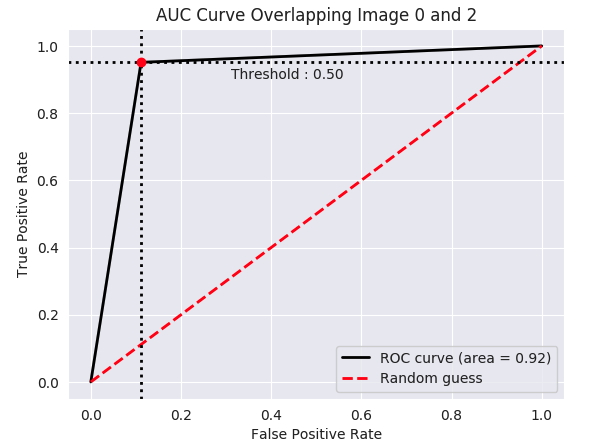
\includegraphics[scale=0.3]{../screenshot/Overlapping/roc01.png}
  \end{center}

  \hspace*{5mm} The random forest machine learning model implemented in databricks for non-overlapping image012 provided insufficent results in terms of numeric
  accuracy and precision measurements. In 4.4 Figure 36, the final training accuracy was 0.93 and testing accuracy was ~0.80. This suggested that the splitting of training and testing data did not provided an equally
  balanced data for the model to use as indicated by the large differences in training and testing accuracy values. Class1 and class2 had a precision rate of 0.74 and 0.76 respectively, while class 0 had a precision rate
  of 0.92. This large differences in precision rate between class0 to class1 and class2 indicate that the model was more biased to class0. This can indicate that the split of training-testing set method may have unintentionally 
  included more dataset from class0 in one of the sets than class1 and class2. The ROC curve in 4.4 Figure 39 and Figure 40 also provided a very low rate of true positive to high false postitive based on the auc value of 0.44 and 0.62
  for class1 and class2 respectively. In 4.4 Figure 38, the ROC curve for class0 was sufficient with a good rate of true postive to false positive as supported by the auc value of 0.78.  
  This large differences in the auc values among class0 to class1 and class2 the models bias towards class0 and thus, it may not be a good model for the three class image classfication. 

  \subsection{Task 3 Figures Non-Overlapping Image012}
  \begin{center}
  \captionof{figure}{Non-Overlaping Image012 Score}
	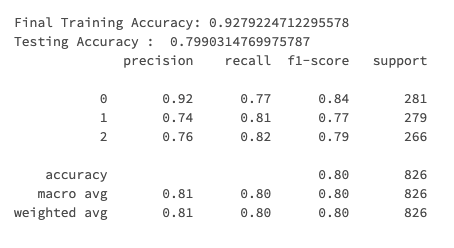
\includegraphics[scale=0.4]{../screenshot/Non-Overlapping/score012.png}

  \captionof{figure}{Non-Overlaping Image012 Confusion Matrix}
	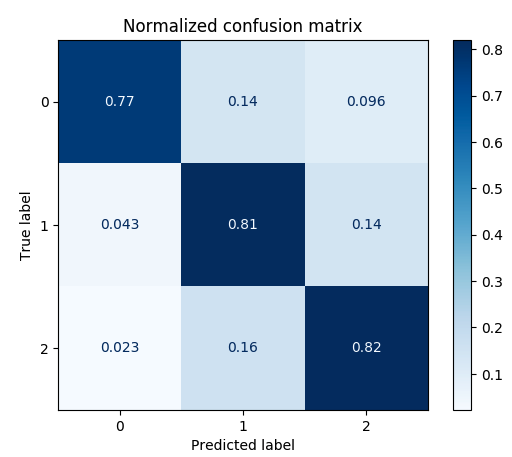
\includegraphics[scale=0.4]{../screenshot/Non-Overlapping/cf012.png}

  \captionof{figure}{Non-Overlaping Image012 Class 0 ROC Curve}
	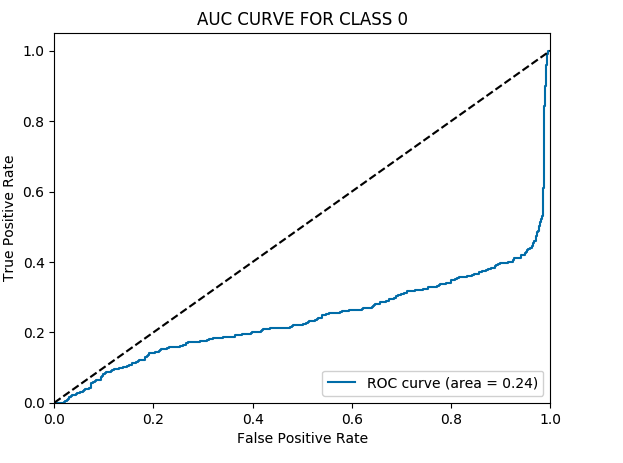
\includegraphics[scale=0.3]{../screenshot/Non-Overlapping/roc_0.png}

  \captionof{figure}{Non-Overlaping Image012 Class 1 ROC Curve}
	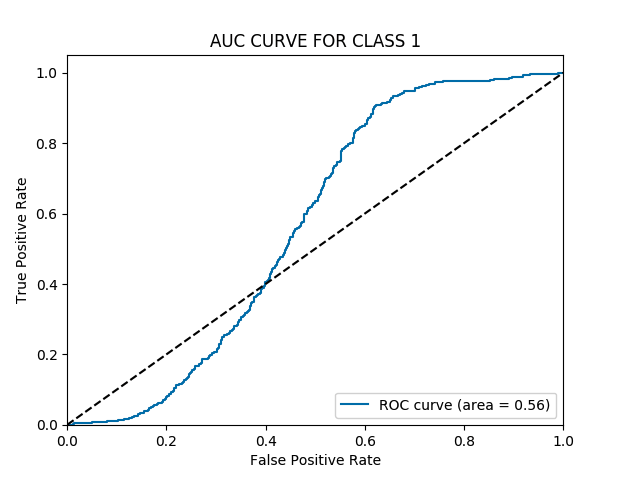
\includegraphics[scale=0.3]{../screenshot/Non-Overlapping/roc_1.png}

  \captionof{figure}{Non-Overlaping Image012 Class 2 ROC Curve}
	\includegraphics[scale=0.3]{../screenshot/Non-Overlapping/roc_2.png}
  \end{center}
 
  \hspace*{5mm} In contrast, The random forest machine learning model implemented in databricks for overlapping image012 provided a sufficent results in terms of numeric
  accuracy and precision measurements. In 4.5 Figure 41, the final training accuracy was 0.95 and testing accuracy was ~0.85. This suggested that the splitting of training and testing data provided a slightly less
  balanced data for the model to use as indicated by the small differences in training and testing accuracy values. Class0, class1 and class2 had a precision rate of 0.95, 0.80, and 0.85 respectively, the result of this
  precision rate indicate that the model might had a small bias towards class0, also performed sufficiently when classify class1 and class2. The ROC curve in 4.5 Figure 43 and Figure 45 also provided sufficient rate of true positive to false postitive based on the auc value of 0.78 and 0.70
  for class0 and class2 respectively. However, in 4.5 Figure 44, the ROC curve for class1 was insufficient as supported by the auc value of 0.58.  
  This large differences in the auc values among class0 and class2 to class 0 as suggested by the ROC curve may suggests that the model is bias towards class0 and  class2.
  Nevertheless, its prediction was sufficient enough to classify the three images as supported by the 4.5 Figure 42 confusion matrix as the true positive rate for class 0, class 1 and class 2 was 0.82, 0.90 and 0.86 respectively.  

  \subsection{Task 3 Figures Overlapping Image012}


  \hspace*{5mm} Overall, the two class model for overlapping and non-overlapping dataset performed significantly better than that of the three class model as it had no bias
  towards one class versus the other class. However, in the scope of the three class model, the overlapping model performed better than the non-overlapping model as it resulted in less
  bias towards any of the three classes. It was also able to predict the three classes sufficiently as supported by the recall rates and the true positive rates for each of the classes shown in the 4.5 Figures.  

  \begin{center}
  \captionof{figure}{Overlaping Image012 Score}
	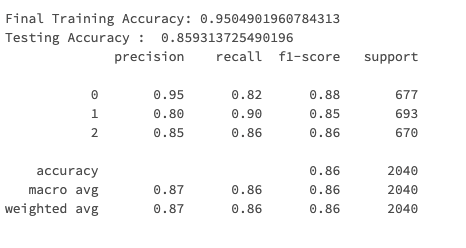
\includegraphics[scale=0.4]{../screenshot/Overlapping/score012.png}

  \captionof{figure}{Overlaping Image012 Confusion Matrix}
	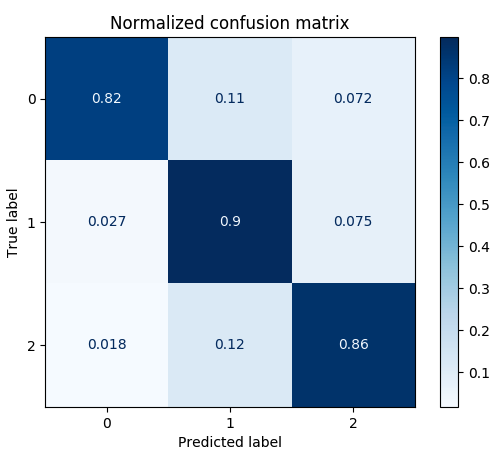
\includegraphics[scale=0.4]{../screenshot/Overlapping/cf012.png}

  \captionof{figure}{Overlaping Image012 Class 0 ROC Curve}
	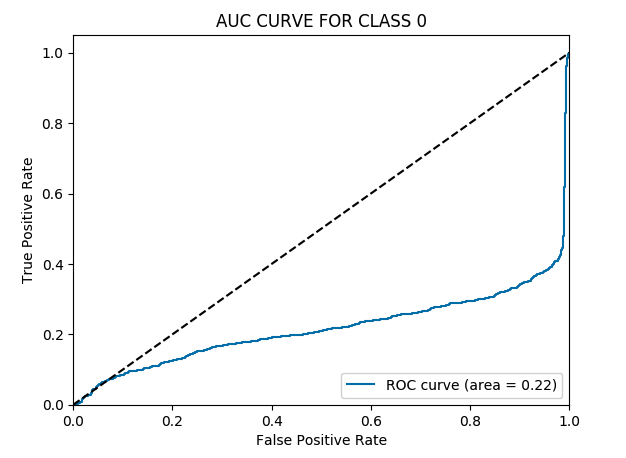
\includegraphics[scale=0.3]{../screenshot/Overlapping/roc_0.png}

  \captionof{figure}{Overlaping Image012 Class 1 ROC Curve}
	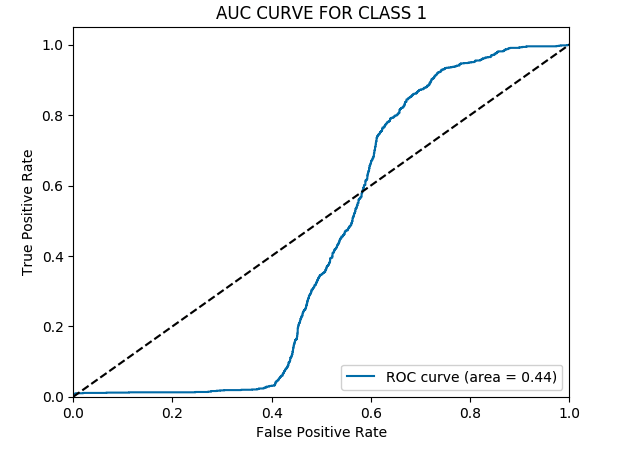
\includegraphics[scale=0.3]{../screenshot/Overlapping/roc_1.png}

  \captionof{figure}{Overlaping Image012 Class 2 ROC Curve}
	\includegraphics[scale=0.3]{../screenshot/Overlapping/roc_2.png}
  \end{center}
  

  \section{Task 4}

  \hspace*{5mm} An overview of the results from the local machine and databricks powered by Amazon Web Services can be found in subsection 5.1 and 5.2 figures. There was quit a noticeable difference
  between the performance speed, when training the random forest model on the local machine in comparison to training in on the databricks platform. When training on the databricks platform, the model took about 
  ~1.5 seconds to train on a full set of features, whereas in the local machine it took aproximately ~3.5 on just half of the features in the dataset. The computing power and performance speed of databricks 
  over performed the local machine. 


  \subsection{Task 4 Figures Local Machine Score}
  \begin{center}
    \captionof{figure}{Non-Overlapping Image01 RF Score}
		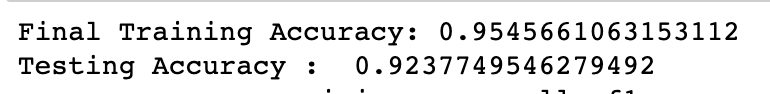
\includegraphics[scale=0.4]{../screenshot/Rf-Non-Overlapping01/score.png}
    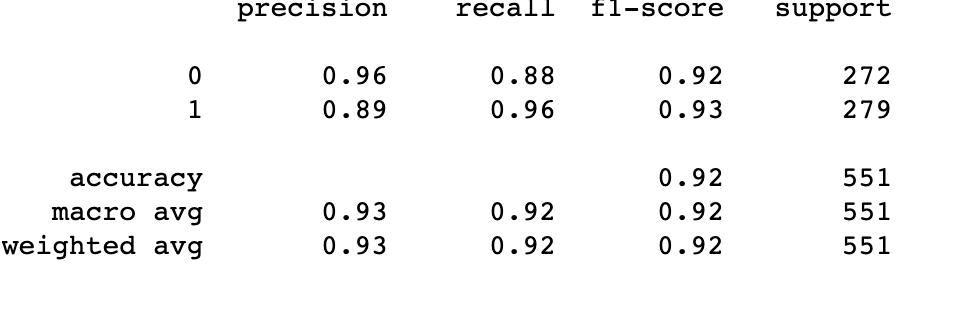
\includegraphics[scale=0.4]{../screenshot/Rf-Non-Overlapping01/machine_score.png}

    \captionof{figure}{Overlapping Image01 RF Score}
		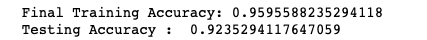
\includegraphics[scale=0.4]{../screenshot/Rf-Overlapping01/score.png}
    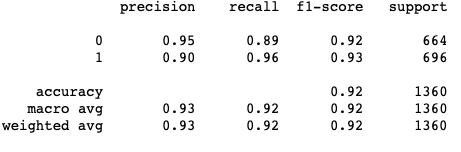
\includegraphics[scale=0.4]{../screenshot/Rf-Overlapping01/machine_score.png}

    \captionof{figure}{Non-Overlapping Image012 RF Score}
		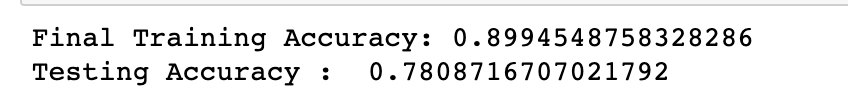
\includegraphics[scale=0.4]{../screenshot/Rf-Non-Overlapping012/score.png}
    \includegraphics[scale=0.4]{../screenshot/Rf-Non-Overlapping012/machine_score.png}

    \captionof{figure}{Overlapping Image012 RF Score}
		\includegraphics[scale=0.4]{../screenshot/Rf-Overlapping012/score.png}
    \includegraphics[scale=0.4]{../screenshot/Rf-Overlapping012/machine_score.png}    
  \end{center}

  \hspace*{5mm} For the comparison of the dervied results of the model, an analysis of their results was done through the scope of the respective model. For the non-overlapping model for image0 and image1, the results
  derived was similar in both the local machine and databricks. In 5.1 Figure 46, the local model scored a training and testing accuracy of 0.95 and 0.89 and the databricks model scored a testing and training accuracy of
  0.96 and 0.89 as shown in 5.2 Figure 50. The predicting precision for class 0 and class 1 was also similar for both models as both scored at 0.96 and 0.89. 

  \hspace*{5mm} For the model of overlapping image for image0 and image1, the results were nearly identical as the testing and training accuracy for both models were aproximately 0.96 and 0.95 respectively as seen in 
  5.1 and 5.2 Figure 47 and Figure 51. The precision rate for class0 and class1 was also identical as both models had a precision of aproximately 0.95 and 0.90 for the respective classes. 


  \hspace*{5mm} As for the model for non-overlapping image for image0, image1, and image2. The databricks model performed slightly better than that of the local model as it scored a 0.92 and 0.80 on the training and testing accuracy based on
  5.2 Figure 52. However, the results were not significantly different enough to warrant a decision in deciding which model was fundamentally better as the local model training and testing accuracy came close with a score of 
  0.78 and 0.90 as shown in 5.1 Figure 48. The precision score of the databricks model for class0, class1, and class2 was also slightly higher with a score of 0.89, 0.74 and 0.73 respectively. However, this did not warrant 
  that the justification that one model was better than the other as the differences in scores was only by a few percentage points.

  \hspace*{5mm} Similary the results for overlapping image for image0, image1, and image2, the databricks model also performed slightly better than that of the local model as it scored a 0.95 and 0.86 on the training and testing accuracy based on
  5.2 Figure 53. However, like the non-overlapping results, it was not significantly different enough to warrant a decision in deciding which model was fundamentally better as the local model training and testing accuracy came close with a score of 
  0.84 and 0.91 as shown in 5.1 Figure 49. The precision score of the databricks model for class0, class1, and class2 was also slightly higher with a score of 0.95, 0.80 and 0.85 respectively. However, this did not warrant 
  that the justification that one model was better than the other as the differences in scores was only by a few percentage points.



  \subsection{Task 4 Figures Databricks Score}
  \begin{center}
    \captionof{figure}{Non-Overlapping Image01 RF Score}
		\includegraphics[scale=0.4]{../screenshot/Non-Overlapping/score01.png}
  

    \captionof{figure}{Overlapping Image01 RF Score}
    \includegraphics[scale=0.4]{../screenshot/Overlapping/score01.png}

    \captionof{figure}{Non-Overlapping Image012 RF Score}
		\includegraphics[scale=0.4]{../screenshot/Non-Overlapping/score012.png}

    \captionof{figure}{Overlapping Image012 RF Score}
		\includegraphics[scale=0.4]{../screenshot/Overlapping/score012.png}  
  \end{center}

  \hspace*{5mm} Overall, the model resulted in a similar accuracy and precision scores from both the local machine and databricks. The only noticeable difference was the large difference
  in precision among the 3 class models. Class 0 had a significantly higher score of precision than that of class 1 and class 2. This inherent problem was consistent in both the local machine and databricks, 
  and therefore can be pin point to the test-training method as it can create an imbalance set that favored class0 and in turn can cause a bias towards class0 in training the random forest models.
  In conclusion, in terms of results, there was not a noticeable difference between that of the models from databricks and local machine. 
  However, in terms of speed and performance, the databricks platform significantly out perform the local models as databricks was able to train the random forest model in an efficient amount of time on a full set of data. 
  The Databricks distributed system handled large sets of data and complex machine learning model well in comparison to the local machine through its speed and efficiency. 



\end{multicols*}

		

	

\end{document}